\section{Data and Preprocessing}
The ODDS-Dataset published by \citet{Rayana:2016} is a widley used repository as benchmark datasets.
E.g. \citet{shenkar2022anomaly} use those datasets to identify stregths and weaknesses of a bunch of outlier detection methods, including the above describes InterCont.
The datasets contain 32 datasets wich different amounts of dimensions and instances. 
To take the whole picture of a method, it is beneficial to use a wide range of different datasets, to determine the advantages and disadvantages of a method.
Nevertheless, using upto 32 different datasets is not feasable for my thesis, because it wont be in the scope of this thesis.
Therefore I will analyse the wine dataset in great detail, to use those finding in the result section.
The goal of this section is to anaylse and describe the dataset.
Therefor I will first summarize the dataset statistically, including central tendencies, shape, distribution, cardinality and spracity.
Subsequently I will analyse bivariate relationships inside the dataset as well.
Finally I will analyse the geomatric structure of the dataset, including intrinsic dimensionality and manifold structure.


The wine dataset was donated from \citet{wine_109} at the 30.06.1991 to the UC Irvibe machine learning Repository.
The authers collected data about chemical components of wine wich came from three different italian wine growers. 
First it was used as a multi classification task dataset, because it had three classes, one for each wine grower.
For outlier detection Shebuti et al tranformed this dataset into an unbalanced binary classification dataset and offered it in the ODDS Repository for general scientific uses. 
129 instances (wines) and 13 variables were left in the remaining dataset.
She combined the wines of wine grower two and three to be the normal class, resulting in 119 wines and wine grower one was defined as the anomaly class, resulting in 10 abnormal wines.
Correspondingly, the outlier ratio is 7,7\% placing it in the \todo{filling the average outlier ratio of ODDS}
Conviently, Shebuto et al excluded all missing data and left only continious instances.
In the following the feature names are not included into the diagrams because of design choices.
Therefor the firgur 1 displays the names of the features: 

%\begin{figure}[h]
%    \centering
%    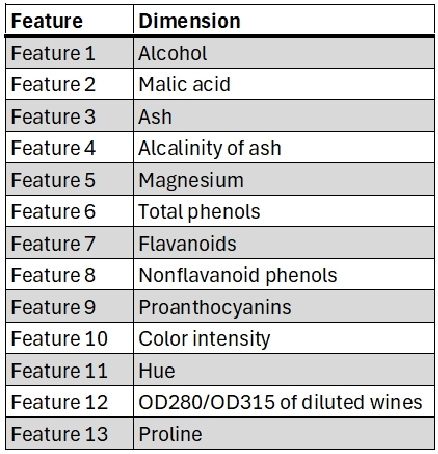
\includegraphics[scale=0.5]{Images/Table_of_Names.pdf}
%    \caption{Featurenames}
%\end{figure}

\subsection{Data Analysis}
In this section  I will describe the central tendencies of the dataset, beginning with univariate analysis.
Figure three is depicting boxplots per feature in the dataset.
The mean, median, interquartile Range (IQR) and the whiskers (1,5*IQD) are displayed.
The red dotted line is the mean and the grey line is the median of the feature.
The mean is not robust against outliers, not like the median. 
The difference between the two parameters can be interpreted as skewdness of the distribution. 
If the mean is bigger than the median, the distribution is right-skewed.
If the mean is smaller than the median, the distribtion is left-skewed.
This is especially pronounced for Malic Acid (Feature 2). 
All of the features are left skewed, except of Feature 8 and 12.
But those differences are not as pronounced as other differences of other features.
That means, that the values of those instances tend to be skewed to major values. 


The IQR dislayes 50\% of the data, that sorrounds the median.
The wider the IQR the bigger the variance of that instance is and vice versa. 
The different features have wide range of boxes. 
While feature 3,4,5 and 6 have a narrow IQR, does feature 12 a peculiar IQR.


If there is no outlier in that instance the wiskers will display the range of the rest of the data.
Like before with the mean-median-comparison, the wiskers display the skewness of the distribution.
If the top wisker is longer than the bottom wisker, the distribution will be right-skewed and vice versa. 
Especially feature 2, 6, 7, 10 and 12 are features that that are skewed to major values.


%\begin{figure}[h]
%    \centering
%    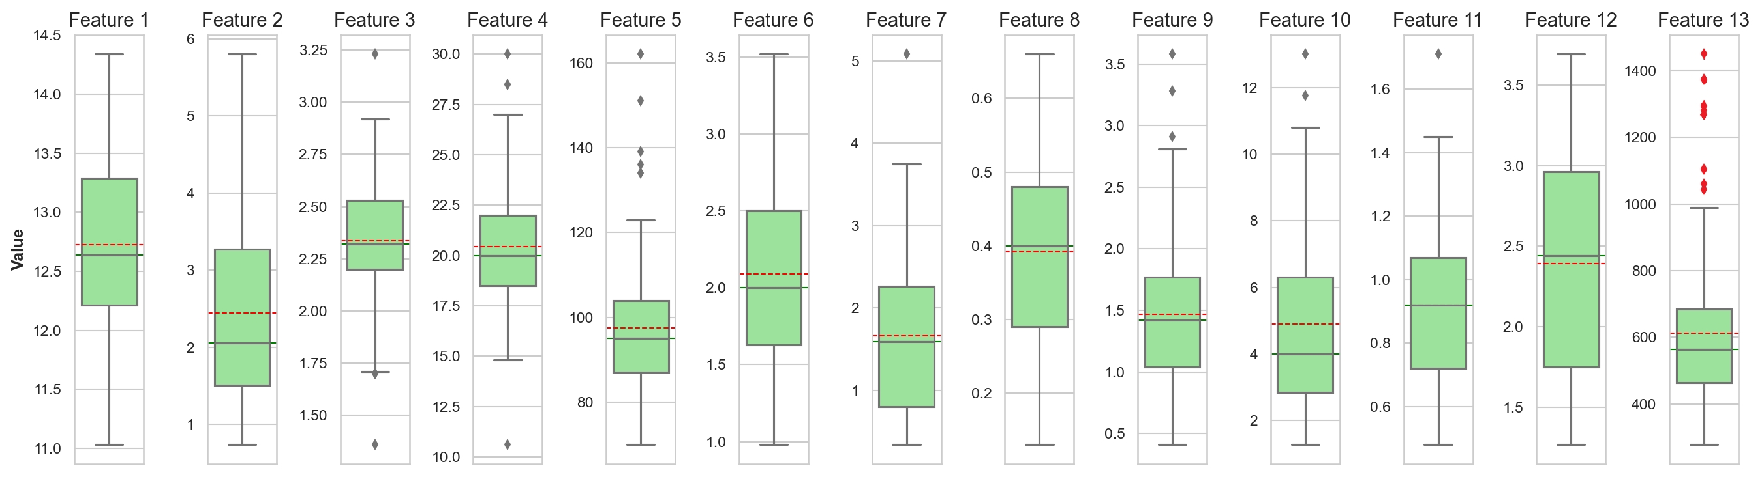
\includegraphics[width=1.0\linewidth]{Images/boxplots.pdf}
%    \caption{Boxplots}
%\end{figure}


Some features contain outlier dotts, that are displayed above or under the wiskers.
A boyplot defines an outlier as an abnormal value of an instances.
That means, that those values can be interpreted as an global outlier.
They are far away from other values in its distibution. 
Only three instances in feature 3 and 4 are outliers because of their minor values.
All the other outliers are defined as outliers because of their major values. 


Boxplots do not include the relationships between variables like its correlations.
To further analyse those outliers, I compared the ground truth with the boxplot outliers.
Some outliers could be defined as outliers, but in fact could be explained by a relationship of another variable. 
Outliers that are boxplot outliers as well as ground truth outliers are coloured in red.
As depicted in figure 3, not all boxplot outliers are in fact outliers.
The boxplot outliers that are not ground truth outliers are wrongly detected, hence false positives.
Depending on the method of treatement, using a boxplot to analyse outliers could have negative side effects on experimental results.


Analysing relationsships between variables, the boxplot can give only hints for the relationships.
For example the boxplot defined 8 instance correctly as outliers, hence the majority of the abnormal class of wine contains a unusually high amount of Proline.
It seems to be a collective cluster in that dimension only, knowing that the dataset contains only 10 outliers in total. 
For that specific data that means, that the wine of the first wine grower has an unusual amount of Proline.
In other dimensions other instances were defined as boxplot outliers, but were not ground truth outliers. 
That means, that the unsusual value of them could be explained by its relationship to other dimensions. 


%\begin{figure}[h]
%    \centering
%    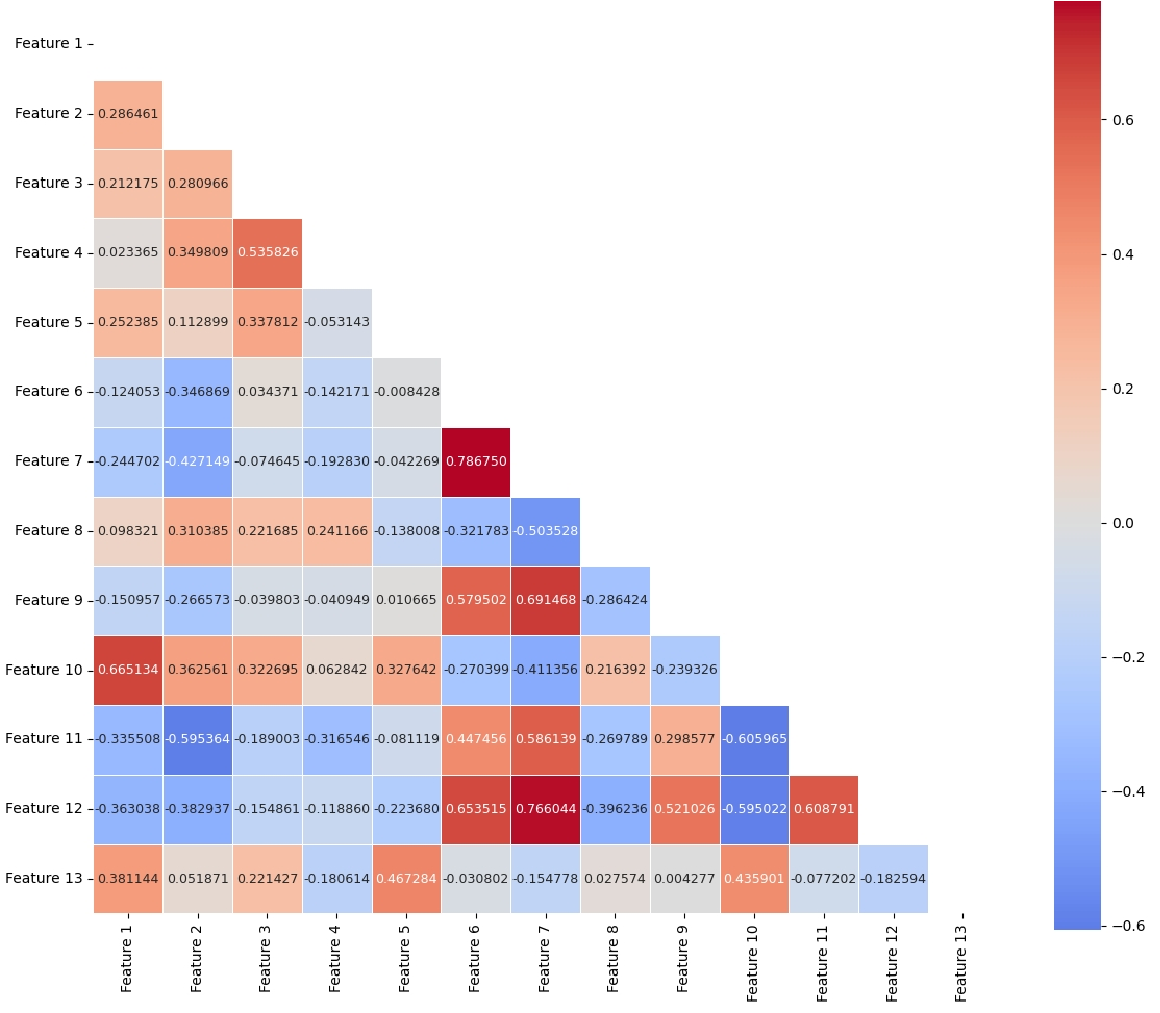
\includegraphics[width=1.0\linewidth]{Images/heatmap.pdf}
%    \caption{Correlation Heatmap between pairs of Dimensions}
%\end{figure}


The correlations between the dimensions vary.
If the coefficient is positive, the movement of the value of feature A is rectified with the value of feature B.
If the coefficient is negative, the movement of the value of feature A is contrary to the movement of feature B's value.
If the coefficient is 0, the value stays the same when the value of feature B shifts.
The dimensions that are the most correlated are total phenols and flavonoids (feature 6 and 7) with a correlation of 0.806292.
OD280/OD350 of diluted wines and flavonoids (feature 12 and 7) are highly correlated as well witch a correlation of 0.772444.
Hue and color intensity are highly negatively correlated with a correlation of -0.639528.
The second most negatively correlated dimensions are OD280/OD350 of diluted wines and color intensity (feature 12 and 10) with a correlation of -0.594243.


Figure 4 is displaying the Pearson correlation between pairs of dimensions.
I chose to display the Pearson correlation because there was no difference between the Spearman and Pearson correlation.
The Spearman correlation is better used in datasets, that have non-linear relationships.
Furthermore it is robust against gloabl outliers, because it ranks the values befor calculating the correlation. 
I calculated both and realized that there is not a difference, implying linear relationships between the dimensions.
Moreover the outliers in the dataset are small enough and the dataset is imbalanced enough, that the coefficient does not change. 
Pearson correlation displays the realtionship between two variabels by assigning a number to it.


As described before, there are hints, that the distribution of the data is slighly skewed. 
To analyse it further, I plotted a Normal Q-Q plot in figure 5 for each feature, to compare the distribution of the data with a normal distribution.
The Normal Q-Q plot is a scatterplot that compares the quantiles of the data with the quantiles of a normal distribution.
If the data is normally distributed, the points in the Q-Q plot will approximately lie on a straight line.
Analysing the figure, non feature is perfectly normally distributed, but some features are more normally distributed than others.
Feature 3 and 4 are the most normally distributed features, because their points are closer to the straight line, except for the last instance, that deviates from the line.
If the ordered valus formed as a bell curve, the data has heavy tails, meaning that there are more extreme values than expected in a normal distribution.
Thats the case for feature 5.
Instances in the first and last quantiles of the feature distribution deviate from the expected normal distribution, indicating that there are more extreme values than expected in a normal distribution.
If the points in the Q-Q plot are formed as a S-shaped curve, the data is skewed to the right or left depending on where the points exceed the normal distirbution line, as seen in feature 7 wich is left skewed.


%\begin{figure}[h]
%    \centering
%    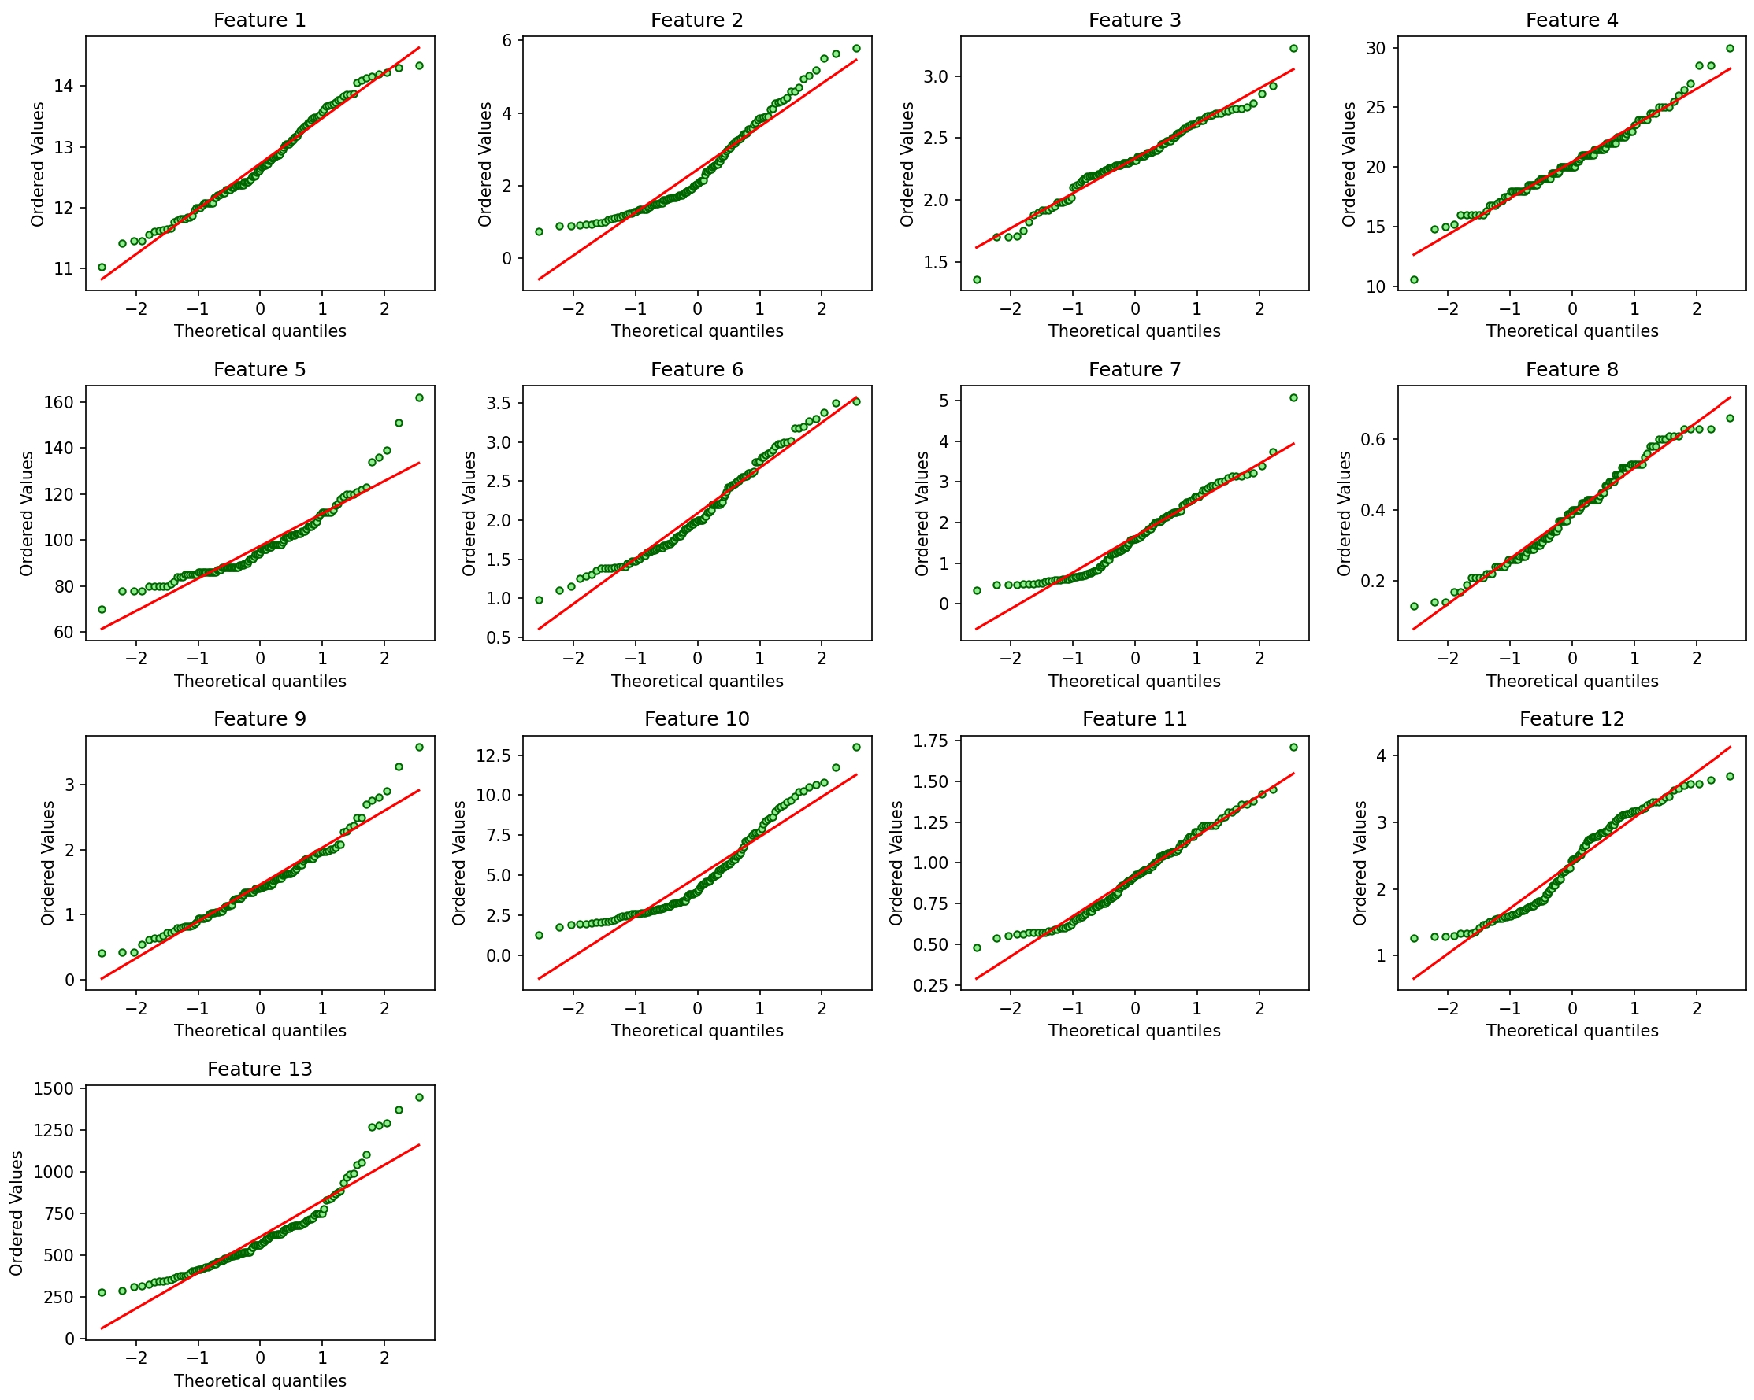
\includegraphics[width=\textwidth]{Images/Q-Q Plot.pdf}
%    \caption{Q-Q Plot for each feature}
%\end{figure}


To be statistically sure, I apply the Shapiro-Wilk test for Normality.

To further analyse the dataset, I will use the Uniform Manifold Approximation and Projection (UMAP) to reduce the dimensionality of the dataset, because it is the standard dimension reduction technique in scientific research.
The goal is to visualise the datasets manifold structure, meaning that the data is clustered or on a curved surface.
UMAP is a non-linear dimension reduction technique that is designed to preserve the local structure of the data, making it ideal for visualizing complex datasets.
It does this by calculate the k nearest neighbors of each instance.
It need this information to determine, if the data is in a more dense cluster or in a more sparse region of the data space.
It drwas a local radius around the k nearest neighbors.
If the neighbor of a given instance is closer compared to other instances, the connection will be defined as strong.
The further away the neighbor is, the weaker the connection is defined. 
The algorithms defines data instances as being seperated if its not in the local radius of each other.
The resulting neighborhood map is integrated into one grapf by simplicial complex.
A scatter plot is generated with same number of instances randomly placed onto it.
Accordingly to the grapf, instances wich are close are pulled together and instances whose connection is weak are pushed appart.
That interation is complete, if a low energy state is reached.

Two main hyperparameters of UMAP has to be defined. 
Those hyperparameters are defining how the visualization is generated, hence there is no definitive correct way to set them.

\begin{enumerate}
  \item Number of Neighbors: This hyperparameter defines the number of nearest neighbors that UMAP will consider for defining a neighborhood
    It sets the focus of the analysis. The trade-off relationsship determines what will be displayed in the visualization 
    If the number is small, UMAP will focus on local structure, but if the number is high, UMAP will focus more on global structure.
   \item Minimum Distance: This hyperparameter controls how tightly UMAP packs points together in the low-dimensional space. 
    A smaller minimum distance will result in a more clustered visualization, while a larger minimum distance will produce a more spread-out visualization.
    If the goal is to determin clusters, it is advisable to set the number of neighbors to a small number, becaus it will focus on local structure. 
    If the goal is to determine the overall shape of the data, it is advisable to set the number of neighbors to a high number, because it will focus on global structure.
    In that case, I want to visualise the overall shape of the data, hence I set hyperparameter to a high number.
\end{enumerate}

I chose the default seetings to create the visualisation. 
The goal was to visualtize, if the dataset has distinct clusters or if the clusters are more blended together.
Therefor I set the number of neighbors to 15 and the minimum distance to 0.1.


The data is normalized by using the Z-score normalization, to ensure that all features are on the same scale and to prevent any feature from dominating the visualization due to its scale.
The Z-Score normalizsation is robust against global outliers, because it uses the mean and standard deviation of the data to scale the features, which are not affected by outliers as much as min-max normalization.
Importantly the axis are not inerpretable, because the UMAP is a non-linear dimension reduction technique, hence the resulting dimensions are not directly related to the original features.
But the distances between the points in the UMAP plot can be interpreted as a measure of similarity between the instances in the original high-dimensional space.


The data instances are colored accourdingly to the ground truth labels.
The red dots are in the outlier class and the blue dots are in the normal class.
Two clusters emerge in the visualization.
The outlier class forms a cluster as well as the normal class is more spread out.
The normal class is put together and therefor it is not possible to define clusters in the normal class.
The outlier class forms a tight cluster, clearly seperated from the normal class.
That is an indication that the outliers are highly distinct.

It is worth noting, that UMAP takes a sochastic approach, meaning that the resulting visualization can change.
After repeatingly changing the hyperparameters, I found that the clusters do not change a lot.
The proof are displayed in the appendix.


In contrast to other dimension reduction techniques, UMAP preserves more global structure.
But measuring exact distances between the clusteres should be analyzed with caution. 


The resulting diagram is displayed in figure 6.
%\begin{figure}[h]
%    \centering
%    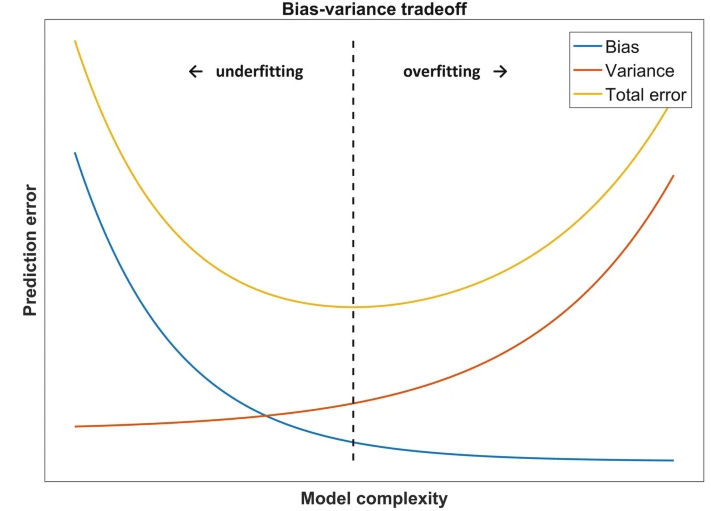
\includegraphics[width=0.5\textwidth]{Images/To_be_implemented/Bias_Variance_Tradeoff.png}
%    \caption{Visualization of the dataset via UMAP}
%\end{figure}



\subsection{Metrics}
Performance metrics are essential for analyzing the success of outlier detection and ensuring that different methods can be compared effectively. 
Selecting the right metrics is a difficult but vital task to ensure the results remain meaningful and consistent. 
This process requires balancing two needs: first, using metrics that are widely accepted by the research community to maintain standard benchmarks; and second, choosing metrics that fit the specific dataset and the unique challenges of outlier detection to avoid misleading conclusions.


An analysis of 276 papers explicitly documenting model performance reveals that the True Positive Rate (TPR)—alternatively referred to as sensitivity, recall, or the detection rate—represents the most frequently utilized metric. 
The TPR quantifies the proportion of anomalous instances correctly identified by the model. 
Complementarily, 116 of the surveyed papers employed the False Positive Rate (FPR), also designated as the false alarm rate, which measures the frequency of benign instances erroneously classified as anomalies.
A critical observation from this literature review is that 64 out of 290 papers relied exclusively on a single performance metric, predominantly Accuracy or the Area Under the Curve (AUC). 
Such a reductive approach is often insufficient for a comprehensive determination of a machine learning model's qualitative performance, particularly in imbalanced domains. 
Beyond predictive efficacy, a significant subset of the literature incorporates computational performance indicators, including CPU utilization, execution time, and specific training or testing durations. 
These metrics are essential for assessing the operational efficiency of an algorithm. 
These findings corroborate the research by \citep[postfix]{nassif2021}, which highlights the ubiquity of TPR while noting that FPR was reported in only 116 of the 290 surveyed studies, alongside a secondary focus on various measures of computational latency.


The confusion matrix is taken as a starting point to derive different scientifically accepted metrix.
I will explain the basic metrics even if they are not often used in outlier detection, because they are commonly known in the research community. 
Thereafter I will go on with more sophisticated metrics, such as the F1-Score, Accuracy and Precision.
In the end I will explain agnostic metrics which are the Area under the ROC-Curve (AUC) and the Area under the Precision-Recall Curve (AUPRC)


\todo{adding: concentrating on binary classification, not multiclass or hierarchical classification, because the datasets I use are binary.}
\todo{adding: explaining why wont use runtime}
\todo{critique other paper wich use not suitabl metrics, }
\todo{explain that a whole framework of metrics has to be implemented, because every metric has its own advantages and disadvantages.}


\subsection*{Confusion Matrix}
A simple way to evaluate the performance of a method, is to apply the confusion matrix to the results. 
Outlier detection, as defined as an imbalanced binary classification problem, can by analysed a traditional 2X2 confusion matrix.
Therefore the results are compared to the ground truth and are sorted into the matrixes cells.
The confusion matrix are constructed as seen in figure.
The horizontal presents the methods hypothesised class and the vertical presents the true class.


%\begin{figure}[h] 
%    \centering
%    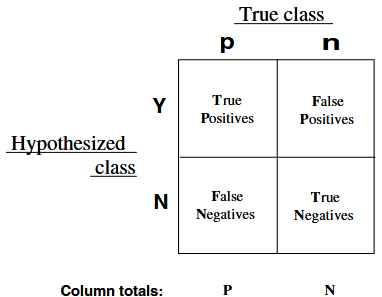
\includegraphics[width=1\linewidth]{Images/Confusion Matrix.pdf}
%    \caption{Confusion Matrics}
%    \label{fig:my_example}
%\end{figure}


The main diagonal represents correctly classified instances.
Outliers that are correctly classified are called true positives, while correctly classified inliers are called true negatives.
The other diagonal presents the falsly classified data instances.
Outliers that are wrongly classified as inliers are called false negatives, while inliers that are wrongly classified as outliers are called false positives.
All basic metrics are derived fromt the confusion matrix \citep[p.4]{saito2015precision}. 
In scientific literature, a heuristic approach is often taken.
All of them need a threshold to seperate outliers from inliers, which is a mayor disadvantage.
In real-world scenarios, the outlier ratio is not known, and therefore need to be calculated from already collected data.
Setting the threshold to high, increases the number of outliers incorrectly classified as inliers.
Setting the threshold to low, increases the number of inliers incorrectly classified as outliers.
Depending on the domain, this might lead to incorrect decisions.  
Especially in unsupervised learning, the outlier ratio is used as the threshold, avoiding an abritrary value selection.
In scientific research this provides a plain level field to compare different outlier detection methods.
The most often used metrics derived from the confusion matrix are:


\enumerate

    \item Accuracy: Measures the overall efectiveness of the method, by calculating the proportion of correctly classified instances to the total number of instances.
    It is defined as:
    
    \begin{equation}
        \text{Accuracy} = \frac{TP + TN}{TP + FN + FP + TN}
    \end{equation}

    The disadvantage of accuracy is that it can be misleading when the method classifies none instance as an outlier, because the dataset is imbalanced.
    If the outlier ratio us very small, the method can classify this small percentage wrong, but achieve a high accuracy, by ignoring the incorrectly classified outliers.

    \item Precision: Measures the proportion of correctly classified outliers (true positives) to the sum of all instances that are predicted as positives, hence correctly and incorrectly classified outliers.
    The focus is the class agreement of the data labels with the positives labels given by the classifier.
    It is defined as: 

    \begin{equation}
        \text{Precision} = \frac{TP}{TP + FP}
    \end{equation}

    The disadvantage of precision is that it can lead to conservative classification behaviour, because the method can optimze by ony classify the most obvious outliers.
    If the method classifies an outlier incorrectly, the denominator will increase, hence the precision will decrease. 
    This metric ignores the false negatives, that will be high, if the method classifies conservatively.
    Thats especially problematic, in high stakes scenarious, where the cost of missing an outlier is high, like in fraud detection or medical diagnosis.

    \item True Positive Rate (TPR) or Recall/Sensitivity: Measures the proportion of correctly classified outliers (true positives) to the sum of correctly classified outliers and false classified inliers.
    The incorrect classified inliers should be classified as outliers.
    It is defined as: 

    \begin{equation}
        \text{TPR} = \frac{TP}{P} = \frac{TP}{TP + FN}
    \end{equation}

    The disadvantage of recall is that it can lead to high number of false positives, because the method can optimize by classifieng all instances as outliers.
    If the method classifies an inlier incorrectly, the denominator will increase, hence the recall will decrease, but if the method classifies an outlier correctly, the numerator will increase, hence the recall increases as well.
    This metric ignores the false positives, that will be high, if the method classifies all instances as outliers.
    A possible bad implementation of recall could be manufacturing, where an outlier could trigger a kill switch, which could lead to high restarting costs.
    Precision and recall share a trade-off relationship. 
    Optimizing the relationship between precision and recall is crucial for evaluating the performance of outlier detection methods, especially in imbalanced datasets.
    This relationship will be explained above and will lead to the definition of the metric: Area under the Precision-Recall Curve (AUCPR).

    \item Specificity: Measures the proportion of correctly classified inliers (true negatives) to the sum of incorrectly classified outliers and correctly classified inliers.
    The focus is on the class of inliers, hence the negatives.
    It's goal is to measure the efectiveness of the method to identify negatives.
    It is defined as:

    \begin{equation}
        \text{Specificity} = \frac{TN}{FP + TN}
    \end{equation}

    \item F1 score: The F1 score is the harmonic mean of precision and recall, creating a metric that incorporates the relationship between both. 
    It is defined as: 
    
    \begin{equation}
    F_1 = 2 \cdot \frac{\text{Precision} \cdot \text{Recall}}{\text{Precision} + \text{Recall}}
    \end{equation}

    By using the harmonic mean, the metric is sensitive to small input values.
    If either precision or recall is low, the resulting metric will be smaller than the traditional mean. 
    Therefore the F1-Score is only high in cases where both recall and precision are high too.
    As mentioned before, the two metrics share a trade-off relationship.
    That means, if the model optimizes one metric, the other will decrease, hence decrease the F1-Score as well.
    By optimizing the F1-Score, the model balances both precision and recall.


    The F1-Score is threshold depending, because its inputs are depending on the threshold as well.
    The choice of this threshold influences both the precision and recall, thereby affecting the F1 score.
    

    A mayor point of critique is that F1-Score ignores the correctly classified inliers (true negatives).
    In outlier detection, the inlier class is the vast majority of your data.
    A metric that ignores how well you identify the normal class is technically providing an incomplete picture of the models performance.
        
        
    The F1-Score treats prescision and recall as equal important.
    In real-world scenarios an equally important trade-off may not align with the cost-benefit analysis.
    Diagnosing an healthy patient with cancer may be not so severe as the opposite way around.
    Classifing an accused criminial as more dangerous as he really is, could lead to a stricter scentence then he deserves. 
    Depending on the domain, the solution is to reqeight the recall or the precision, resulting in for example the F2-Score (weighing Recall higher) or F0.5-Score (weighing Precision higher).

\citep[p.430]{sokolova2009systematic}
\endenumerate
\todo{consider: maybe its better to plot this as a table}

\subsection*{Metrics absence of thresholds}
The above explained metrix have in common, that they depend on a threshold value.
To bypass the threshold selection, alternatively one can use the Area und der ROC Curve (ROC AUC) and the Area under the Precision-Recall Curve (AUPRC)


\subsection*{Metrics based on Area under the Curve}
\todo{insert FPR}
The ROC AUC is an aggregate measurement of performance across all possible classification thresholds and it ranges between 0 and 1.
Therefore it can be interpreted as a probability that randomly chosen outlier gets a higher outlier score than a randomly chosen inlier.
The higher the value is, the better the model distinguishes between outliers and inliers.
As seen in the figure, ROC AUC is plotting the true positive rate (TPR) at the ordinate against the false positive rate (FPR) at the abscissa, and can be mathematically expressed as an integral. 
Visually, the higher the ROC AUC is, the more the curve bends outwards to the point (0;1), hence ROC AUC = 1.
At this point the FPR is minimal and the TPR is maximal.
If ROC AUC = 0.5, the model guesses like a coin flip, which defines a baseline for analysing a models performance.
Visually represented by a linear rising graph.
If  ROC AUC = 0 the model classifies outliers as inliers and vice versa perfectly.
Therefore the graph bends to the poin (1;0). 

\todo{insert ROC AUC diagram}

ROC AUC is a good choice for imbalaced classification tasks, like outlier detection, because it evaluates the models ability to rank a ranomd outlier higher than a random normal point.
It does this by incorporating the trade-off relaitonship between precision and recall and does not simply optimize for one class.
Espacially in unsupervised outlier detection, where outlier scores are produced by the methods, ROC AUC can be benefitial, because it does not require a threshold.
Furthermore, ROC AUC is scale invariant and just requieres a consistent ranking of the outlier scores. 
Thats means, that ROC AUC is suitabele for comparing different methods, that are producing different types of outlier score scales. \todo{is that right? Example}


ROC curve is one of the strongest metrics used to efficiently assess intrusion detection systems performance, and it is a graphical tool that illustrates accuracy across FPS \citep[postfix]{nassif2021}
A comprehensive evaluation of classifier performance can be obtained by the ROC insert ROC equation denotes the conditional probability that a data entry has the class label C. 
An ROC curve plots the classification results from the most positive to the most negative classification. 
Due to the wide use in cost/benefit decision analysis, ROC and the Area under the Curve (AUC) apply to learning with asymmetric cost functions and imbalanced data sets


ROC AUC as advantages in inbalaed datasets, but has disadventages, too.
Especially in inbalased datasets, ROC AUC can be over optimistic, because it includes the the FPR.
The number of true negative instances are a lot higher than the true positives. 
The denominator is dominated by the true negatives. \citep{davis2006relationship} 
The change in the FPR by misclassifying inliers, will not be substantial. 
Therefore the FPR tends to be small in inbalaced datasets, hence the curve biased to the left corner.


In defence of ROC AUC, authors \todo{insert paper} argue, that the metric measures the fundamental desciminative power of a model, not like precision-based metrics (e.g. F1-Score)
It stays consistent, even if the outlier ratio changes, what makes it suitable for models comparisons. 
\todo{discuss if the argument is valid}



The area under the precision-recall curve (AUPRC) resolves the argument of the overly optimistic ROC AUC.
Therefore the AUPRC ignores the true negatives and focussing on the models main task: detecting true positives.
As mentioned above, precision and recall share a non-monotonic trade-off relation as well.
Small fluctuation can occure, therefore in the literature the average precision is applied. 
If one metric increases, the other will decrease.
In other words, there is a trade-off between every outlier found (recall) and detecting it correctly (precision)
The AUPRC lays between 0 and 1, with 1 as the pefect model.
Pefect in the sense that it detects all outliers correctly.
As shown in the figure, the diagram plots the recall curve at the abscissa and precision at the ordinate.
The better the performance of a model is, the more the graph bends towards the right corner of the diagram.
The curve declines, because of the ranking of outliers. 
The most obvious outliers are at the top of that list.
If the threshold is very strict, the most obvious outliers are defined as one and most probably correct.
Resulting in a high precision and low recall.
If the threshold is lowered, the the more likely it is, that outliers are incorrectly classified, decreasing precision and increasing recall, bending the curve to the bottom left corner.
\todo{insert citation etc, see davis2006relationship}
\todo{insert paper saito2015precision, difference between ROC and AUPRC}


The AUPRC does not have a fixed baseline, instead it depends on the analysed data and is the outlier ratio.
As a baseline, suppose a naive model with no discriminative power.
This model randomly guesses the outlier ratio in the given dataset varying the threshold.
The probability that the model will predict a true positive is the prevelance of the share of outliers in the dataset (outlier ratio).
The more linient the threshold gets, the more likely it will detect higher number of true positives, increasing recall.
Precision will stay the same, because however the threshold is set, the prevelance of outliers is constant.
Therefore the increasing number of true positives is proportional to the increase of false positives, resulting in a horizontal line.


This framework makes it possible to compare the performance of different methods. 
If the performance of model A is always better than the performance of model B, the graph of model A will always be above the graph of model B.
If the graphs cross each other, then the one model will be better suited for high precision tasks and the other for high-recall tasks.


If the models curve is at this line, the model is guessing which instances is an outlier.
That means, that AUPRC is not suitable to compare methods across different datasets. 


\subsection*{adding: Runtime}


I will conclude this chapter by summarizing the advantages and disadvantages of the metrics explained above before deciding which specific metric I will use in my analysis and explaining the reasoning behind that choice.
Accuracy, Precision, Recall, and Specificity are all calculated from the simple values of the confusion matrix; however, if the classification threshold is changed, the values within the confusion matrix must change as well.
Accuracy is a commonly used metric in outlier detection, with a survey of 290 papers on machine learning-based anomaly detection finding that 112 of those studies utilized Accuracy as a primary metric. \citep[p.78664]{nassif2021}
Nevertheless, Accuracy is fundamentally unsuitable for outlier detection tasks because these datasets are imbalanced in nature. 
The minority class of outliers is much smaller than the majority class of inliers, meaning the impact of the outliers is mathematically reduced. 
For a small given percentage of outliers, Accuracy can be estimated as very high simply by classifying all instances as inliers, resulting in a low percentage of misclassified instances that masks the failure to find any anomalies. 
Therefore, as noted by \citet[p.8]{branco2016survey}, a metric used for imbalanced datasets must consider the actual distributions of the classes.


Precision attempts to negate this problem by ignoring the distributions and the count of true negatives, but this approach has its own disadvantages. 
By ignoring the negatives, a method can optimize for Precision by classifying too conservatively and predicting only the most obvious outliers. 
In contrast, Recall is mathematically cheap to maximize, as an algorithm can achieve a perfect score of 1.0 simply by labeling every single data point as an outlier. 
A model that flags everything is technically perfect according to Recall but is practically useless because it provides zero discrimination between classes. 
Because the count of false positives is entirely absent from the Recall equation, a high-recall model in a business context—such as fraud detection—might flag thousands of legitimate transactions as fraudulent. 
The cost of investigating these false alarms is often high, but Recall does not reflect this noise. 
This makes it difficult to conclude that one method is better than another based on Recall alone without checking for a corresponding surge in false alarms. 
Furthermore, Chicco and Jurman (2020) argue that because Recall ignores two quadrants of the confusion matrix, it provides an incomplete and potentially biased summary of model quality. 
This is particularly problematic for unsupervised outlier detection algorithms that produce continuous anomaly scores, as lowering the threshold can artificially inflate Recall, making fair comparisons difficult without a threshold-independent metric like ROC-AUC or PR-AUC.


Specificity focuses entirely on the negative class, but in outlier detection, the number of true negatives is usually massive. 
Because the denominator is dominated by this high count of inliers, even a significant absolute number of false positives will not noticeably move the metric. \todo{right paper?} \citep{saito2015precision} 
Since Specificity tells the researcher nothing about the model's ability to find actual outliers, a model that labels everything as an inlier will achieve a perfect score despite being a total failure at detecting anomalies.
\todo{add ROC AUC and AUPRC}
\todo{Write this passage specifically for my dataset}

For these reasons, I have chosen to use [Insert your chosen metric here] for my analysis, as it provides a more robust and honest evaluation of performance in the face of extreme class imbalance and varying thresholds.


\subsection{Experiments}
This chapter is about the technical destails of the experiments.
Therefor I will describe the experimental setup and analyse the the arcitecture of the methods, hence the code.
The goal is to supply an indepth understanding of the implementation and the technical details to fulfill a reproduction of my results. 


\subsubsection*{Experimental design}
The experiments are run on a Desktop PC, equiped with a NVIDIA GeForce RTX 3090 and a 12th gen Intel(R) Core(TM) i9 - 12900k 3.2 GHz CPU.
The PC has 65536 RAM and 24326 MB of VRAM. 
It runs Windows 11 Enterprise Version 25H2.
For the code to implement I used the latest version of the integrated development environment (IDE) PyCharm 2025.3.3.
I used python 3.12, because there werent all the packages available for the latest version of python.
I used a virtual environment to manage the dependencies of the project and created a requiremtents.txt file to list all the packages and their versions.


\subsubsection*{InterCont}
The authers of the InterCont method, supplied a reproduction package with their paper. 
The reproduction of the InterCont method went flawlessly and I could reproduce the results of the paper.
Nevertheless, the authers did not include code for other methods, supposably because they are widely used and implemented in standard libraries.
Therefore I implemented the k-NN and MCD methods by myself.


The reproduction package contained 4 different python-files: main, train, data\_loader and helper\_functions.
Beginning with main.py, this file orchestrates the experiment. 
It handles the configuration, load the data and triggers the training process.
Those configurations can be changed by the command line.
I run the code without any command line arguments, so I used the default configurations.
The different configurations are batch size, dataset and faster version.
The default batch size is 3000, which will perform for my relatively small dataset a full batch gradient descent.
The default configuration of 3000 was supposedly chosen by the authers, because in the dataset repository are datasets with more dimensions and instances.
Later I will perform a sensitivity analysis on the batch size, because it is an important hyperparameter for the training process and it can have a significant impact on the results. 
\todo{insert batch size into theory}


The dataset can be changed in the command line argument.
The reproduction package contains all datasets odf the ODDS repository. 
Because I am analysing just one dataset and this dataset happens to be the default setting, I neither use it or change the setting.
The last configuration is the faster version, which I neither use, nor change, because my dataset is relatively small and the default setting is "no" for not implementing the fast version.
 

At the end of the file, the authors implemented a command to ensure that the GPU is primarly used and if it is not avaiable, the processed is been run on the CPU.
Which is also implemented in the train.py file. 
That file determines the training process of the InterCont method.
In the beginning of the file, a datapipeline is been implemented by a datawrapper. 
There the data is determined how many rows a dataset has and how to grab a row. 
For analysing the calculated anomaly score, the wrapper keeps the index names.
The machine learning algorithm then can assign the anomaly score to the right row.


The next encoder class describes the architecture of the method and determines the neural network.
The F network is defined in the following lines beginning with line 28 until line 35.
For the input layer it takes the d-kernel\_size features and puts then through the Tanh activation functionm, resulting in a width of -1 and 1.
The kernel\_size is a hyperparameter, that defined in line 86 until 94. 
Depending on the number of dimensions of the dataset, the kernel\_size is set to 2, 10 or d-150. 
My dataset has 13 dimensions, so the kernel\_size is set to 2.
The hdn\_size refers to the hiddensize argument.
Hiddensize determines how many neurons are in the hidden layers.
Here the hiddenlayers are hardcoded to 200 in line 87. 


The first hidden layer is defined in line 31.
It is defined as an fully connected layer and takes all 200 output values from the previous layer as inputs.
The inputs are projected to double the number of outputs, hence 400 neurons.
Temporarily expanding the dimensionality of the dataset to find non-linear relationships.
The LeakyReLu activation function with its hyperparameter set to 0,2 is implemented in line 32.


The output layer the results from the previous layer is compressed to the predefined hiddensize, hence 200 neurons. 
Because of the compression, the neural network is forced to learn the most important relationsships.
The LeakyReLu is once again implemented.


The smaller G-Network is desigened the same.
From line 38 to line 45 the architecture of the G-Network is defined.
The difference between F and G are in the sizes.
The G network uses the complementary kernel\_size and the number of neurons are divided by 4. 
This network uses only LeakyReLu activation functions.
The hyperparameter stays the same for all activation functions.
The number of neurons are again doubled in the first hidden layer, hence the hiddensize is divided by 2.
\todo{fill in the normalization}

Going ahead, the contrastive 


This method does not implement an cross validation procedure to avoid overfitting. 
Instead they use a permutation based approach to determine the anomaly score.
The dataset is spilt into 50\% training and 50\% testing data.
The training data include only the data from the normal class, while in the test data they include the abnormal data with the normal data. 
This approach is called semi-supervised learning.
To reach the goal of stable and reliable results, the authors implemented a shuffle procedure.
The train and test data stays the same all the time.
But inside this datasets, the order of the columns are being changed, hence shuffeld.

To get randomness into the shuffle process, the authors used the pytorch function torch.randomperm()
This function uses a pseudo-random number generator, hence there is no argument set, the default engine has been used.

The authors tun the code 500 random splits and so did I.
The authors did not provide a loop, so I coded it by myselve.
I did not want to loop the main.py, because then the PC hab to load the data for every loop. 
I applied the semi-supvervised approach in dataloading procedure in the logic of my loop.
I sat the random\_state to 42.
That is a often chosen value in scientific research to ensure reproducability.
I could not tell, if the authors hab chosen another value.  
The metrics are calculated accourdingly to the helper functions.


In the helperfunction\_py is the code for calculating the F1-score.
Here the threshold is not hardcoded as in my other methods.
Instead it is a dynamically coded that meany that the ground thruth lables are incorporated into the threshold calculation.
Then the model takes the threshold and applies it to the sorted outlier ratios.
By comparing the taken instances to the ground truth, the method calculates Precision.
But the number of items picked are equal to the number of actual outliers, Precision equals Recall, hence the F1-score equals the same. 


The authors took k-NN as an classic machine learning algorithm benchmark.
Unfortunately they did not provide in their reproduction package any code to test their results.
Therefore I decided to code my own basic k-NN algorithm to benchmark a machine learning method.
To make the methods comparable I decided to implement a semi-supervised learning approach into the k-NN as well.


\todo{insert arguments why semi supervised can be allpied}

\subsubsection*{k-NN}
The k-NN algorithm is implemented by using the PyOD library, wich is a widely used library for anomaly detection in sientific research.
I also used parts of the well known library scikit-learn to implement the cross validation procedure and to calculate my desired metrics.
First I seperated the dataset into the test and training dataset.
I split the data into same-sized training and testing datasets.
Similiar to the InterCont Method, I put in the normal data into the training dataset and the normal plus abnormal data into the test dataset.


Next the cross validation procedure is implemented by using the KFold function from scikit-learn.
The KFold function takes the number of folds as an argument, which I set to 5.
I chose a 5 fold cross validation approach, because my dataset has not many instances. 
By choosing a relatively small amount of folds, I can ensure that the training dataset is not too small and the testing dataset is not too small as well.
I also set the shuffle argument to True, which means that the data will be shuffled before splitting it into folds.
The random state argument is set to 42, which is a commonly used value in the scientific community to ensure reproducibility of the results.


I sat the contamination parameter to 7,7\%, reflecting the outlier ratio.
That ensures, that the threshold for determining the anomaly score is set to reasonable value grounded on scientif literatur.
The  method parameter determines the distance metric used to calcilate the distances between the data points.
I chose the default setting "largest" which means the distance is calcultate the Minkowski distance with p=2 wich is mathematically equivalent to the Euclidean distance.
The test data is normalized by using the min-max-normalization.


\subsubsection*{MCD}
The FAST-MCD algorithm is also implemented by using the PyOD library. 
I chose an unsupervised learning approach for the MCD algorithm, because it is not possible to implement a semi-supervised learning approach for this method.
Because of its statistical nature, the MCD algorithm does not have a training phase, but it calculates the anomaly score based on the whole dataset.
Therefore I did not implement a cross validation procedure for the MCD algorithm, because it is not possible to split the dataset into a training and testing dataset.
The contamination parameter is also set to the outlier ratio of 7,7\%.
The random state argument is set to 42. 
This ensures that the results are reproducible, because the FAST-MCD algorithm takes random initial subsets and performs the C-Steps thereafter.
By choosing a random state, the reproduction of the results is ensured, because the same random subsets will be chosen in each run of the algorithm.


The authors code is written to implement a high number of different datasets.
My dataset is a .mat-file wich is the dataloader is in part about.
But there 
A lot of code is not necessary to implement my dataset, but I want to keep it, because redundant code will not negatively influence my results.
The interesting thing is, that the hyperparameters are hardcoded and those values are for datasets with more dimensions and instances.
Therefore in the nextchapter I will perform sensitivity analysis on chosen hyperparameters.
Moreover the authors implemented just the F1 and AUC metrics, which I also want to analyse, but I want to analyse the AUPRC as well.
So I made small adjustements to their code which is for transparency reasons marked.

